\documentclass{article}
\usepackage{graphicx}
\usepackage{float}

\begin{document}

\title{Technical Questions and Answers in Machine Learning}
\author{ONI Olalekan Joseph}

\maketitle

\section{Problem 2 **COMPLETED**}
Determine the first and second derivative with respect to $x$ of: $f(x)= \frac{1}{1 + e^{-x}} $

\subsection{Solution to Problem 2 }
 First Derivative: \\
 $$f(x) = (1 + e^-x)^{-1}$$ \\
 Using Chain Rule \\
 $$f'(x) = -1(1 + e^{-x})^{-2} \times -1e^{-x}$$ \\
 $$f'(x) = \frac{e^{-x}}{(1 + e^{-x})^{2}}$$ \\ \\
 
\noindent Second Derivative:  \\
 $$f'(x) = \frac{e^{-x}}{(1 + e^{-x})^{2}}$$ \\
 Using Quotient Rule of Differentiation \\ \\
 $g(x) = e^{-x}$  \qquad  $h(x) = (1 + e^{-x})^{2} $ \\\\
 $ g'(x) = -e^{x} $ \qquad $h'(x) = -2e^{-x}(1 + e^{-x}) $ \\
 $$f''(x) = \frac{h \times g' - g \times h' }{g^2} $$ \\
 $$f''(x) = \frac{-e^{-x} \times (1 + e^{-x})^{2} \enspace + \enspace 2e^{-2x} \times (1 + e^{-x})}{e^{-2x}} $$\\
 $$f''(x) = \frac{e^{-2x} - 1}{e^{-x}} $$
 
\section{Problem 3 **COMPLETED**}
 If I break a stick of unit length into three random pieces, what is the expected length of the largest piece? (You may need to state the assumptions that you make.)
 
\subsection{Solution to Problem 3}
Let the stick be broken at two points $X$ and $Y$. \\
Therefore, we have two independent random variables $X$, $Y$ which are both uniform in [0,1]. \\
Let $A=min(X,Y)$, $B=max(X,Y)$ and $C=max(A,1-B,B-A)$. \\ \\
Let $f_{C}(a)$ be the probability density function (pdf) of C and $ F_{c}(a)$ be the cummulative distribution function (cdf). Then: 

$$ F_{c}(a) = P(C \le a) = P(A \le a, 1-B \le a, B-A \le a)$$
The cdf for the unit square is then equivalent to: \\\\
\[F_{c}(a) = \left\{
\begin{array}{lr}
(3a-1)^2 & : \frac{1}{3} \le a \le \frac{1}{2} \\\\
1-3(1-a)^2 & : \frac{1}{2} \le a \le 1
\end{array}
\right.
\]

Then the pdf is: \\\\
\[f_{c}(a) = \left\{
\begin{array}{lr}
6(3a-1) & : \frac{1}{3} \le a \le \frac{1}{2} \\\\
6(1-a) & : \frac{1}{2} \le a \le 1
\end{array}
\right.
\]
\\
Therefore, the expected length of the largest piece (C) is: \\\\
$$\int_{\frac{1}{2}}^{\frac{1}{3}} 6a(3a-1)da + \int_{1}^{\frac{1}{2}} 6a(1-a)da = \frac{11}{18}$$


\section{Problem 8 **COMPLETED**}
What are the values of the constants $a$, $b$ and $c$ if one writes the following expression in the form: $ a(x - b)^{2} + c$ \\ 

 \begin{equation}\label{key}
 3x^{2} - 4x + 5
 \end{equation}
 
\subsection{Solution to Problem 8}
$$ 3(x^2 - \frac{4}{3}x + \frac{5}{3})$$ \\
$$ 3 \Big[ (x - \frac{2}{3})^2 -\frac{4}{9} + \frac{5}{3} \Big] $$ \\
$$ 3 \Big[ (x - \frac{2}{3})^2 + \frac{11}{9} \Big]  $$ \\
$$ 3 \big(x - \frac{2}{3}\big)^2 + \frac{11}{3}  $$ \\
$ a =3; \enspace b= \frac{2}{3}; \enspace c= \frac{11}{3} $

\section{Problem 6 **COMPLETED**}
A factory that makes light bulbs contains three machines. The machines manufacture 20\%, 30\% and 50\% of the total production. From their production, 5\%, 4\%, and 2\% respectively are faulty. I choose a collection of light bulbs at random from the output.

\subsection{Solution to Problem 6a}
If the collection contains two faulty light bulbs, what is the probability that they come from the same machine? \\\\
Let $P_{M_{Af}}$ represent Probability of faulty bulbs produced from the first machine (A). \\ \\
Similarly for second machine and third machine we have $P_{M_{Bf}}$ and $P_{M_{Cf}}$ respectively. \\ \\
$P_{M_{Af}} = \frac{5}{20}$; \enspace $P_{M_{Bf}} = \frac{4}{30}$; \enspace $P_{M_{Cf}} = \frac{2}{50}$. \\ \\

Let the probability that two faulty light bulbs from a collection come from the same machines be $P_{M_{2f}}$. \\\\
$$P_{M_{2f}} = \Big( \frac{5}{20} \times \frac{5}{20}\Big) + \Big( \frac{4}{30} \times \frac{4}{30}\Big) + \Big( \frac{2}{50} \times \frac{2}{50}\Big) = 0.00163$$

\subsection{Solution to Problem 6b}
Let the probability that the three faulty light bulbs from a collection come from the different machines be $P_{M_{3f}}$. \\\\
$$P_{M_{3f}} = \Big( \frac{5}{20} \times \frac{4}{30} \times \frac{2}{50} \Big) = \frac{1}{750}$$

\section{Problem 4 **COMPLETED**}
The twenty-first century began on 1 January 2001 (a Monday) and will end on 31 December 2100 (a Friday). What percentage of twenty-first century Wednesdays fall on the last day of a month? (This question requires some coding.)

\subsection{Solution to Problem 4}
The Python code snippet is shown in Figure 1. Percentage of the 21st century Wednesdays that fall on the last day of the month: \\\\
$$ = \frac{172}{5242} \times 100 \% $$
$$ 3.3\%  \textit{(1dp)}$$


\begin{figure}[H]
	\centering
	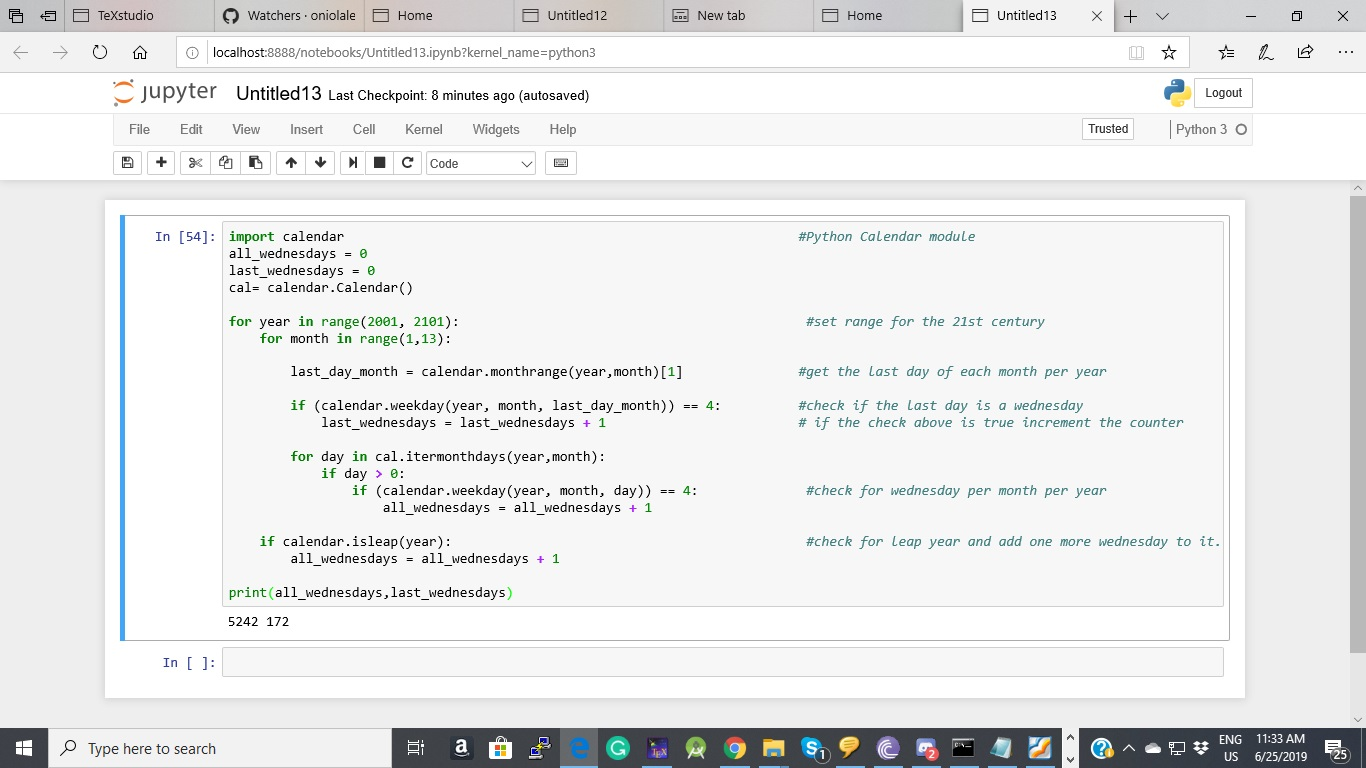
\includegraphics[width=1.2\linewidth, height=0.6\textheight]{pythonCode2}
	\caption{Python Source Code Screenshot}
	\label{fig:pythoncode}
\end{figure}





\end{document}